\chapter{Teoretická část}

Teoretická část práce bude zaměřena na obecné principy, na kterých pracují nejčastější senzory pro monitoring ovzduší. Převážná část z~použitých senzorů využívá nepřímý způsob měření námi požadovaných veličin, kde se většinou změna dané veličiny projeví na senzoru změnou odporu a~tím i~napětí či proudu jím protékajícím.

\section{Měření koncentrace prachových částic}

Prachové částice je možné rozdělit do několika kategorií podle jejich velikosti. Často se lze setkat s~pojmem např. PM2.5, což je zkratka z~anglického particulate matter (pevné částice) a~číslo, které udává maximální velikost těchto částic v~\SI{}{\micro\metre}. Nejčastěji se měří částice do velikosti \SI{10}{\micro\metre}, \SI{2,5}{\micro\metre} a~\SI{1}{\micro\metre}. Částice o~velikosti \SI{10}{\micro\metre} nejsou pro lidský organismus příliš škodlivé, lidské tělo jich většinu dokáže zachytit již při vstupu do dýchacích cest. Problém nastává při vyšší koncentraci částic menších než \SI{2,5}{\micro\metre}. Zde již tělo nemá přirozenou obranu a~dostávají se tak přímo do plic. Částice menší než \SI{0,5}{\micro\metre} jsou schopny proniknout až do krevního řečiště.

Nejčastěji se v~praxi měří koncentrace částic o~velikosti \SI{10}{\micro\metre} a~\SI{2,5}{\micro\metre}. Všechna zařízení pro měření těchto částic fungují na principu pohlcování či odrážení světelného paprsku. Pro měření je tedy potřeba zdroj světla a~detektor světelného paprsku. Jako zdroj se používají LED nebo stále častěji laser. Princip měření tedy spočívá v~osvícení vzorku vzduchu daným paprskem světla, který se o~prachové částice ve vzorku rozptýlí nebo pohltí. Množství dopadeného světla je tedy nepřímo úměrné koncentraci prachových částic v~daném vzorku. V~principu jsme schopni měřit tak malé částice, jak přesný zdroj světla (šířka paprsku) jsme schopni vyrobit a~také jej potom detekovat.

Dříve používané LED mají nevýhodu v~tom, že vyzařují široký paprsek světla, který nejsme schopni jednoduše soustředit do jednoho bodu. Lze využít optickou soustavu pro zaostření takového paprsku světla, ovšem v~daném prašném prostředí by docházelo k~častému opotřebení a~zaprášení čoček, které by poté ztrácely své vlastnosti a~měření by bylo nemožné. Z~těchto důvodů je v~dnešní době více používanější laser, jelikož jsme schopni vytvořit paprsek o~dané vlnové délce, výkonové hustotě a~velikosti. 

Poslední součástí těchto detektorů je mechanismus, kterým se do senzoru dostává čerstvý vzorek vzduchu. Nejjednodušší je využití malého ventilátoru, který bude do prostoru senzoru vhánět čerstvý vzduch z~okolí. Nevýhodou takového řešení je hlučnost senzoru a~také možnost zanášení senzoru nečistotami z~okolí. Proto se objevují i~senzory, které mají tento ventilátor nahrazený topným elementem (nejčastěji výkonový rezistor), kterým protéká proud a~ohřívá vzduch okolo, viz obrázek \ref{fig_dustSensorPrinciple}. Ten pak díky rozdílné hustotě teplého a~studeného vzduchu začne stoupat vzhůru a~unáší s~sebou prachové částice do měřeného prostoru. Zde je ovšem třeba dávat pozor na konstrukci takového senzoru a~na výrobcem předepsané požadavky na montáž, jelikož jej nelze umístit téměř libovolně v~prostoru, jako tomu může být u~senzoru s~ventilátorem \cite{teor_DustSens, teor_PMMeas}.

\begin{figure}
    \centering
    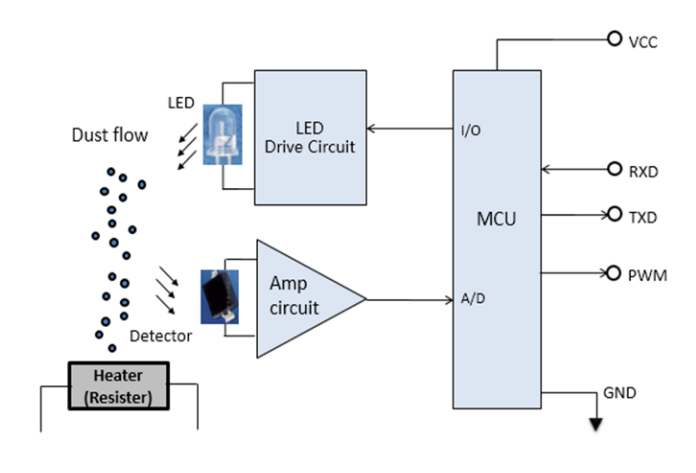
\includegraphics[width=0.70\textwidth]{obrazky/dustSensorPrinciple.png}
    \caption[Blokové schéma senzoru prachových částic PM1003.]{Blokové schéma senzoru prachových částic PM1003 \cite{PM1003Datasheet}.}
    \label{fig_dustSensorPrinciple}
\end{figure}

\section{Měření oxidu uhličitého}

Oxid uhličitý (CO$_2$) je plyn běžně se vyskytující v~zemské atmosféře a~jeho koncentrace kolísá na základě hned několika faktorů. Lokální hodnoty může ovlivňovat například výskyt mnoha živočichů či lidí na jednom místě. V~globálním měřítku má ale na svědomí tzv. globální oteplování, jelikož jeho koncentrace v~atmosféře díky lidské činnosti rok od roku stále roste. Sám o~sobě v~malém množství není pro lidi nebezpečný, ale se zvyšující se koncentrací má za následek zpočátku bolesti hlavy, přecházející v~utlumení nervových soustav a~zhoršeného dýchání až po koncentraci 20~\%, kdy může způsobit i~smrt \cite{teor_COMeas}.

\subsection{Optický senzor}

Oxid uhličitý lze měřit více způsoby. Nejpřesnější možností je optický senzor využívající infračervené světlo. Tento typ senzoru je založen na základě měření rozdílu intenzity infračerveného záření o~dané vlnové délce. Přiváděný plyn je osvětlován infračerveným zářením, které je přítomnými molekulami oxidu pohlcováno a~poté je přes reflexní vrstvu odraženo zpět do snímače, kde je umístěn pyrodetektor, který převádí intenzitu tohoto světla na elektrický signál. Se vzrůstající koncentrací klesá intenzita světla dopadajícího na povrch pyrodetektoru. Tento princip měření je nejpřesnější, podává stabilní výsledky a~má dlouhou životnost. Bohužel je velice drahý, a~tak jej není možné použít v~domácích zařízeních \cite{teor_COMeas}.

\subsection{Elektrochemický senzor}

Tento druh senzoru pracuje na principu měření proudu vznikajícího reakcí sledovaného plynu s~elektrolytem, který je obsažen uvnitř senzoru. Při konstrukci takovéhoto senzoru je třeba zvolit elektrody a~elektrolyt tak, aby na jedné z~elektrod docházelo k~chemické reakci, která vyvolá změnu proudu. Tato změna je následně zesílena do měřitelné podoby, a~odpovídá koncentraci oxidu uhličitého. Bohužel díky nutnosti chemické reakce několika přítomných látek není tento druh senzoru možné zkonstruovat pro dlouhou životnost. Spolu s~tímto neduhem je zde také časová nestálost podávaných výsledků kvůli ubývání elektrolytu a~opotřebení měřících elektrod. Životnost takového senzoru je tedy maximálně v~řádu několika málo roků \cite{teor_COMeas}.

\subsection{Polovodičový senzor}

Poslední a~zároveň nejlevnější možností měření koncentrace oxidu uhličitého je použití polovodičových senzorů. Polovodičový přechod u~těchto senzorů je vyroben tak, aby se při přítomnosti sledovaného plynu změnila jeho vodivost. Na základě této změny jsme poté schopni změřit napětí a~proud na přechodu, čímž můžeme určit koncentraci CO$_2$. Nevýhodou těchto systémů je jejich relativní nepřesnost a~hlavně nelineární průběh měřeného signálu. Jsou ovšem díky své ceně snadno použitelné a~dostupné v~komerčně prodávaných detektorech do domácností a~pro laická měření. Pro exaktní měření je ovšem nutná jejich častější kalibrace vůči známé koncentraci měřeného plynu \cite{teor_COMeas}.

\section{Měření intenzity osvětlení}

Intenzita osvětlení se měří na základě fotoefektu. To znamená, že při dopadu elektromagnetického záření na látku dojde k~uvolnění elektronů z~této látky a~naopak k~pohlcení fotonů. Nejčastěji se pro tento jev používají polovodiče.

\subsection{Fotodiody}

Prvním z~používaných typů senzorů jsou fotodiody. U~nich se využívá vnitřního fotoelektrického jevu, který je pro polovodiče typický. Dopadem fotonů na PN přechod fotodiody dochází ke zvyšování procházejícího proudu diodou. Tento proud jsme schopni následně měřit a~vyhodnocovat. Fotodiody mají výhodu v~jejich rychlé odezvě na skokovou změnu a~citlivosti.

\subsection{Fototranzistory}

Dalším často používaným prvkem pro měření intenzity osvětlení jsou fototranzistory. Zde se využívá nejčastěji bipolární tranzistor NPN, který má volnou bázi. Při výrobě jsou konstruovány tak, aby fotony dopadly do oblasti báze a~způsobily tak zvýšení protékajícího proudu tranzistorem. Díky tomu, že se díky fotonům řídí proud do báze tranzistoru, tak je tranzistor na světlo více citlivější než fotodioda. Nevýhodou fototranzistoru je shora omezené spektrum detekovaného světla a~jeho pomalá reakce. 

\section{Měření UV záření}

Měření UV (ultrafialové) záření probíhá v~principu úplně stejně, jako měření intenzity osvětlení. Jediným podstatným rozdílem je vlnová délka záření, na které jsou dané senzitivní součástky nejvíce citlivé, viz obrázek \ref{fig_UVLight}.

\subsection{UVA záření}

UVA záření je nejčastěji se vyskytující záření, které má rozsah vlnových délek mezi \SI{315}{\micro\metre} do \SI{400}{\micro\metre}. Toto záření je zcela běžně přítomné všude kolem nás, jelikož dokáže projít zemskou atmosférou. Při běžném kontaktu s~tímto zářením nám nehrozí žádné zdravotní problémy, ale nedoporučuje se trvalejší vystavení tomuto záření. Běžně se také využívá při procesech luminiscence či různých světelných efektech. Lidské oko jako takové jej není schopné vnímat, narozdíl od některých zvířat.

\subsection{UVB záření}

Dalším z~UV záření, se kterým se můžeme setkat, je UVB záření s~vlnovou délkou od \SI{280}{\micro\metre} do \SI{315}{\micro\metre}. Toto záření je pro živé organismy zhoubné, jelikož dokáže rozkládat bílkoviny. Při dopadu do lidského oka dokáže způsobit oslepnutí, neblahý efekt má též na rostliny, u~kterých ovlivňuje fotosyntézu, a~také způsobuje jejich úhyn.

\subsection{UVC záření}

Posledním z~těchto záření je UVC záření, které je, se svou vlnovou délkou menší než \SI{280}{\micro\metre}, nejtvrdším z~těchto záření. Při kontaktu s~kyslíkem začíná vznikat ozon a~je silně karcinogenní pro všechny živé organismy. Díky své krátké vlnové délce dokáže proniknout relativně hluboko do všech organických materiálu a~je tak velice nebezpečné \cite{teor_UVMeas}.

\begin{figure}
    \centering
    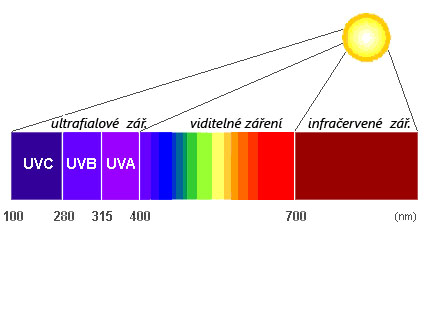
\includegraphics[width=0.7\textwidth]{obrazky/uv_light.jpg}
    \caption[Rozdělení záření podle vlnové délky.]{Rozdělení záření podle vlnové délky \cite{picture_UVLight}.}
    \label{fig_UVLight}
\end{figure}

\section{Měření teploty}

Teplota je základní veličinou, která se dá ve spojitosti s~ovzduším měřit. Pro tento účel se často používají materiály, které spolu s~měnící se teplotou mění svůj odpor. Dvě nejčastější skupiny těchto materiálů jsou kovy a~polovodiče. Kovy mají většinou kladný teplotní koeficient odporu, což znamená, že se vzrůstající teplotou roste i~jejich odpor. Naopak druhou často používanou skupinou materiálů jsou polovodiče, které mají negativní teplotní koeficient, a~tak jejich odpor s~rostoucí teplotou klesá.

\subsection{Kovové senzory}

Pro potřeby obecného měření lze využít odporové senzory vyrobené z~kovů. Vyznačují se poměrně vyrovnanou charakteristikou a~také vysokým teplotním rozsahem. Tyto senzory se dále dělí na NTC (Negative Temperature Coefficient) a~PTC (Positive Temperature Coefficient), podle toho, jestli mají negativní teplotní koeficient, nebo pozitivní. Například platinové teplotní čidlo je možné použít pro velký rozsah teplot, přibližně od \SI{-200}{\celsius} do \SI{800}{\celsius}. Mezi jejich hlavní výhody patří již zmíněná linearita a~odolnost při vysokých teplotách. Nevýhodami jsou nutnost přesného zpracování signálu díky menší citlivosti a~také jejich tepelná kapacita, díky které nejsou schopny rychle reagovat na změnu teploty.

\subsection{Termočlánky}

Další z~možností měření, založené na kovech, jsou termočlánky. Ty pracují na základě Seebeckova jevu, kde při spojení dvou různých kovů dochází při změně teploty k~vygenerování malého napětí, které jsme schopni po zesílení dále měřit. Jejich velkou výhodou jsou malé rozměry a~odolnost i~při relativně vysokých teplotách (tisíce~\SI{}{\celsius}). Jsou tedy vhodné do aplikací, kde je potřeba velký rozsah teplot a~zároveň jsme limitováni maximálními rozměry.

\subsection{Polovodičové senzory}

Polovodiče obecně jsou závislé na teplotě, takže je lze použít pro měření teploty. Jejich charakteristika ovšem většinou není lineární a~závisí na Shockleyho rovnici:
\begin{equation}
    I_A =I_S \cdot (\mathrm{e} ^{\frac{U_A}{n \cdot \frac{k \cdot T}{q}}} - 1),
    \label{eq_Shockley}
\end{equation}
kde $I_{A}$ je proud procházející polovodičem, $I_{S}$ je saturační proud, $q$ je elementární náboj elektronu, $U_{A}$ je difúzní napětí, $n$ je emisní koeficient, $k$ je Boltzmannova konstanta a~$T$ je teplota přechodu polovodiče.

Nejvíce lineární, a~zároveň časově stálou závislost na teplotě, má varikap. Pro orientační měření (např. sepnutí aktivního chlazení) lze použít i~diodu či tranzistor, který se umístí na společný chladič s~výkonovými prvky a~následně lze díky změně proudu jimi procházejícím řídit následnou logiku.

Díky stále dokonalejším výrobním procesům pro integrované obvody lze integrovat teplotní senzory přímo na čip. Přímo na tomto čipu tak může být nejen teplotní senzor, ale i~např. operační zesilovač či řídící čip pro digitální komunikační rozhraní \cite{teor_TempMeas, teor_TempSens}.

\section{Měření vzdušné vlhkosti}

Vzdušná vlhkost je přítomná všude okolo nás, a~je definována jako množství nasycení vzduchu vodními parami. Sledovat tuto veličinu je důležité jednak pro člověka, ale i~kvůli elektronice a~jiným strojům. Uvažujeme-li teplotu \SI{0}{\celsius} a~malou vlhkost, bude to pro nás mnohem příjemnější, než stejná teplota a~vlhkost téměř \SI{100}{\percent}. Pro elektroniku a~stroje je poté vlhkost důležitá kvůli jejímu správnému fungování, případně můžou při vysoké vlhkosti začít vodní páry kondenzovat a~způsobit zkrat či při dlouhodobém působení výrazně urychlit oxidaci materiálů.

Její měření se většinou realizuje pomocí součástek založených na principu kondenzátorů. Taková součástka má dvě pevné elektrody, na kterých jsme schopni měřit napětí a~také dielektrikum, které je realizováno pomocí materiálu, který je schopen absorbovat molekuly vody. Tímto způsobem jsme tedy schopni ovlivnit výslednou kapacitu daného kondenzátoru. Při nasycení dielektrika vodními parami se změní kapacita, což jsme schopni změřit a~vyhodnocovat. Toto nasycení je poté úměrné vodním parám obsaženým v~měřeném prostředí. Běžně se jako dielektrikum používají plasty či polymery s~dielektrickou konstantou 2 až 15 \cite{teor_HumSensor, teor_CapacitiveHum}.

\section{Měření atmosférického tlaku}

Pro měření atmosférického tlaku se nejčastěji používá měřidel založených na principu vytlačování kapaliny do předem známého prostoru se stupnicí vlivem působící síly. Měřidla založena na těchto principech jsou v~meteorologii stále hojně používána díky jejich jednoduchosti a~velmi vysoké přesnosti. Ovšem takováto měřidla se hodí jen pro ruční odečítání, jelikož je nelze nijak zautomatizovat.

\subsection{Piezoelektrické senzory}

Jednou z~možností, jak vyrobit elektronický senzor na měření tlaku, je využít piezoelektrického jevu. Tento jev se vyskytuje nejčastěji v~krystalech křemíku, kde při působení síly (v tomto případě atmosférického tlaku) je díky mírné deformaci krystalu vygenerováno velice malé napětí, které úměrné aplikované síle. Toto napětí jsme schopni po adekvátním zesílení jednoduše změřit a~pokud známe strukturu použitého krystalu, tak i~zpětně přepočítat na původní působící tlak.

\subsection{MEMS senzory}

V dnešní době jsou velice rozšířené tzv. MEMS (Micro Electro Mechanical Systems) senzory. Jsou založeny na principu spojení mikro-mechanického principu s~elektrickým principem. Nejčastěji je pro měření tlaku při tomto principu využíváno vlastností kondenzátorů či piezoelektrického efektu.

Při využití principu kondenzátoru je jedna z~elektrod pevně spojená s~pouzdrem, a~následně je druhá elektroda upevněna nad tuto první, tím vznikne kondenzátor, jak je vidět na obrázku \ref{fig_memsCapacitiveSensor}. Druhá elektroda je mechanicky vyrobena tak, aby měla přístup k~okolnímu prostoru a~mohl na ni tudíž působit okolní atmosférický tlak. Díky jeho působení se začne prohýbat a~přibližovat druhé elektrodě, čímž se mění celková kapacita tohoto kondenzátoru a~tu jsme schopni následně měřit a~na jejím základě určit působící atmosférický tlak \cite{teor_PresSens}.

\begin{figure}
    \centering
    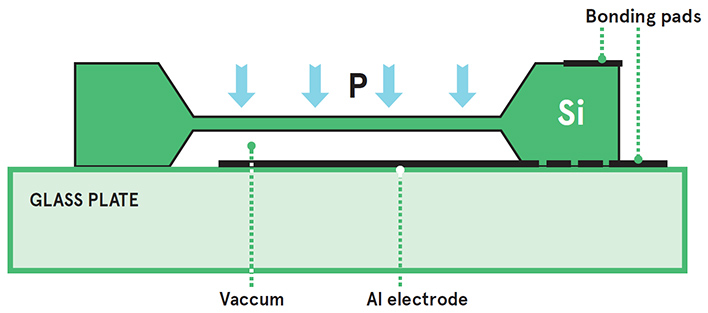
\includegraphics[width=0.7\textwidth]{obrazky/MEMS_capacitive_sensor.jpg}
    \caption[MEMS kapacitní senzor tlaku.]{MEMS kapacitní senzor tlaku \cite{AvnetMEMS}.}
    \label{fig_memsCapacitiveSensor}
\end{figure}

\section{IoT sítě}

IoT (Internet of Things) sítě jsou uzpůsobeny pro přenos relativně krátkých datových zpráv na velmi velké vzdálenosti a~to vše při zachování nízké spotřeby. Dosah je většinou určen podle nosného kmitočtu, na kterém přenos funguje, podle dostupné šířky pásma pro náš přenos a~také vhodně zvolenou modulací. Tyto sítě se většinou nazývají jedním sdruženým pojmem LPWAN (Low Power Wide Area Network). Do této kategorie se řadí především technologie LoRa, Sigfox a~NB-IoT. První dvě zmíněné pracují v~bezlicenčním pásmu, kdežto poslední využívá licenční pásmo. Bezlicenční pásma jsou u~nás regulovány ČTÚ\footnote{Český telekomunikační úřad \url{https://www.ctu.cz/}} a~jejich omezení zpravidla spočívá v~maximálním vyzářeném výkonu a~také klíčovacím poměru. Ten určuje, jaké maximální procento daného času smíme použít pro vysílání. V~následujících částech práce se budu věnovat těmto třem sítím podrobněji.

\subsection{LoRa}

LoRa (Long Range) je fyzická vrstva, kterou využívá síť LoRaWAN a~jak již bylo zmíněno, je určena v~Evropě převážně pro provoz v~bezlicenčním ISM pásmu \SI{868}{\mega\hertz} (dnes je možný přenos i~v~pásmu \SI{2.4}{\giga\hertz}). Tato vrstva samotná je využitelná pro komunikaci mezi dvěma zařízeními bez existence jakékoli sítě. Mnohem častěji ale narazíme na zapojení všech komunikujících zařízení do jednotné sítě, která všechna zařízení sdružuje a~umožňuje tak pokrytí mnohem většího území. LoRa využívá CSS modulaci (Chirp Spread Spectrum), která umožňuje zvýšení dosahu oproti například FSK modulaci. Využívá se rozptrostřeného pásma pro šíření signálu, což jej činí odolným proti rušení. Protože je využito těchto rozprostřených frekvencí, tak je signál i~odolný vůči vícecestnému šíření. Na obrázku \ref{fig_chirpSpreadSpectrum} je vidět příklad průběhu amplitudy rozloženého spektra v~závislosti na čase.

\begin{figure}
    \centering
    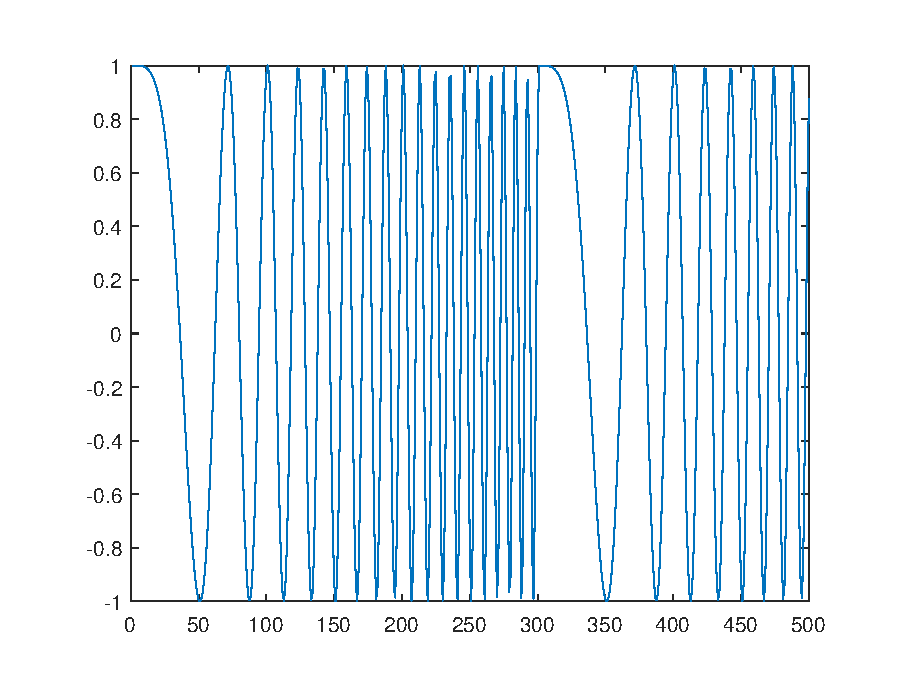
\includegraphics[width=0.8\textwidth]{obrazky/ChirpSpreadSpectrum.eps}
    \caption{Ukázka průběhu rozprostřeného spektra v~čase.}
    \label{fig_chirpSpreadSpectrum}
\end{figure}

\subsection{LoRaWAN}

LoRaWAN definuje princip komunikační sítě a~také použitý protokol, pro svou komunikaci využívá již výše zmíněnou fyzickou vrstvu LoRa. Nejčastěji se využívá zapojení sítě do hvězdy, což umožňuje jednoduše škálovat dostupnost sítě. Pro fungování sítě je potřeba server, který bude zpracovávat všechny příchozí zprávy a~následně na ně reagovat, dále jsou třeba jednotlivé tzv.~gateway, což jsou zařízení, na které se připojují koncoví klienti (naše IoT zařízení). Ná obrázku \ref{fig_LoRaWANNetwork} je vidět příklad zapojení takovéto sítě. Je patrné, že koncová zařízení nemají pevně přiřazenou gateway na kterou se mají připojit, ale vysílají signál, který následně může přijmout libovolný počet těchto bran. Server, který tyto přijaté zprávy zpracovává, tak musí filtrovat případné duplicitně přijaté zprávy. Tím, že zařízení vysílá zprávu "do neznáma"{} a~nemusí řešit přihlašování k~přístupovému bodu, případně do sítě, tak se tím zkracuje doba potřebná k~vysílání a~vede to k~další úspoře energie.

V dnešní době je čím dál tím víc nutné zajistit bezpečnost takto přenášených zpráv. U~LoRaWAN je využit šifrovací algoritmus AES (Advanced Encryption Standard), kdy je po celou dobu přenosu zprávy od koncového zařízení až na aplikační server, který data zpracovává, jím zpráva zašifrována.

Pro připojení zařízení lze využít existující komerčně nabízené sítě od např. Českých Radiokomunikací\footnote{\url{https://www.cra.cz/pripojeni-k-iot-siti-lorawan}} nebo open source sítě provozované komunitou, kde nejznámější je TTN (The Things Network)\footnote{\url{https://www.thethingsnetwork.org/}}. I~v~této komunitní síti však platí omezení, pokud chceme síť využívat zdarma. Jsme limitování na maximální vysílací čas \SI{30}{\second} pro uplink a~maximálně 10 zpráv na downlink pro jednu node (zařízení) na den \cite{TTN_fair_use}. Hlavní výhodou však je možnost přidat vlastní gateway a~poskytovat tak připojení nejen pro sebe, ale i~pro ostatní uživatele v~okolí.

\begin{figure}
    \centering
    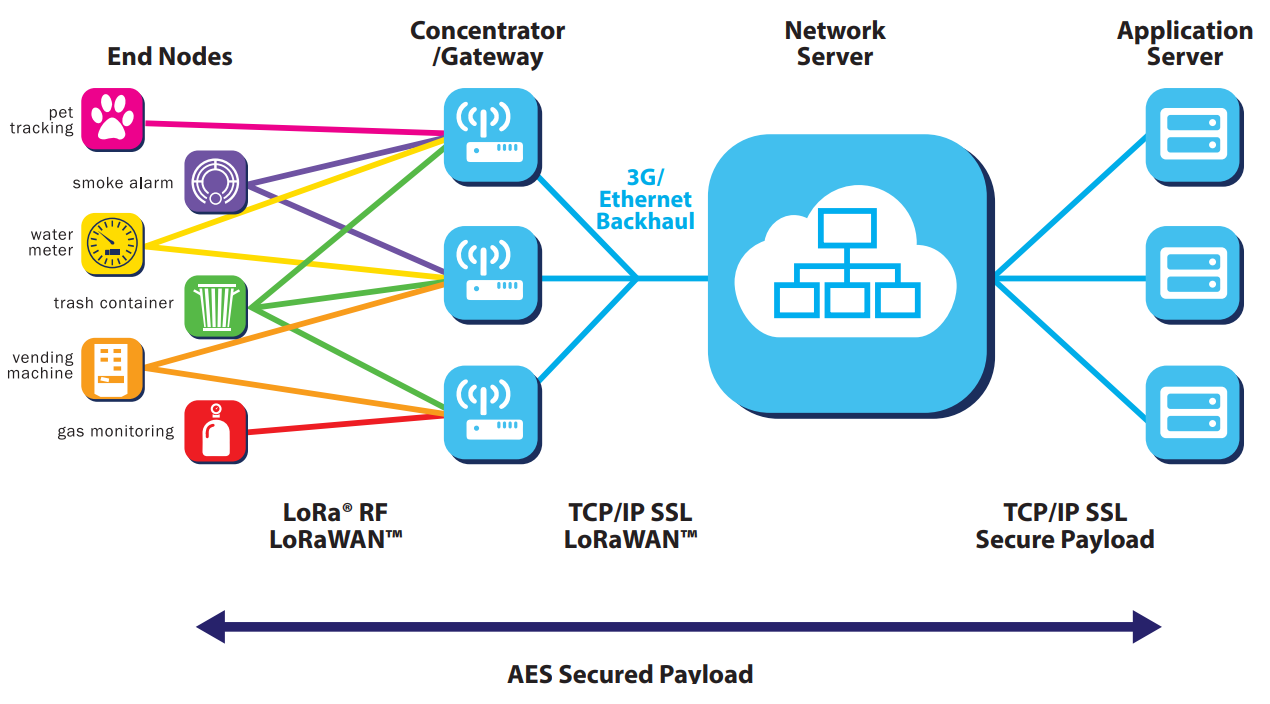
\includegraphics[width=0.95\textwidth]{obrazky/lorawanNetwork.png}
    \caption[Typické zapojení LoRaWAN sítě.]{Typické zapojení LoRaWAN sítě \cite{LoRaWAN_pdf}.}
    \label{fig_LoRaWANNetwork}
\end{figure}

\subsection{Sigfox}

Síť Sigfox pochází z~Francie a~je docela podobná technologii LoRaWAN. Je opět určená pro malý přenos dat ze sledovaných zařízení skrze nelicencované frekvenční pásmo. Oproti LoRaWAN má ovšem nevýhody a~to, že je třeba za přenos zpráv platit poskytovateli a~provozovateli sítě. Síť totiž u~nás spravuje jediný poskytovatel\footnote{SimpleCell Networks a.s. (\url{https://sigfox.cz/cs})}, ke kterému se musíme zaregistrovat a~on nám poté poskytne připojení a~přenos zpráv skrze jeho síť. Výhoda tohoto řešení může být v~mnohem větším pokrytí daného území a~odpadnutí nutnosti řešit vlastní gateway či server na zpracování přijatých dat.

Přenos u~nás probíhá v~pásmu \SI{868}{\mega\hertz} se šířkou spektra \SI{192}{\kilo\hertz}, kde každý kanál má přiřazenou šířku \SI{100}{\hertz}. Vysílání zpráv probíhá na třech kanálech s~drobným časovým odstupem, čímž se zvyšuje šance na zachycení takto vyslané zprávy. Pokrytí na našem území je zajištěno ve spojení s~operátorem T-Mobile, čímž dosáhli umístění gateway na strategická místa. Dle jejich webových stránek uvádí pokrytí území v~květnu 2022 \SI{94}{\percent} rozlohy ČR \cite{Sigfox_pokryti}.

\subsection{NB-IoT}

Síť NB-IoT (Narrowband Internet of Things) je LPWAN síť, kde její standardy definuje partnerský projekt 3GPP \cite{3GPP}. I~u~tohoto typu sítě je opět snaha minimalizovat velikosti posílaných zpráv, mít co největší dosah a~to vše za udržení minimálních energetických nároků. Díky tomu, že lze síť provozovat na již existující infrastruktuře LTE vysílačů, je zde možnost velmi rychlé implementace a~její nasazení na velké oblasti, stačí totiž softwarová aktualizace vysílačů. U~nás tuto síť provozuje mobilní operátor Vodafone právě v~pásmu LTE. Síť NB-IoT využívá pouze \SI{200}{\kilo\hertz} pásmo a~tak může existovat vedle již existujících sítích pro mobilní telefony. V~důsledku použití licencovaného pásma nejsme omezeni na vysílací čas a~také je možné vysílat mírně vyšším výkonem, než v~bezlicenčním pásmu ISM. Je však nutné mít podporovaný modul od operátora a~vlastnit jeho SIM kartu pro připojení do sítě. Bohužel momentálně není možné získat tyto SIM karty pro nekomerční využití, nabízí je totiž jen firemním zákazníkům. 

Do budoucna mají tyto sítě velký potenciál právě díky jejich rychlému nasazení a~využití stávajících sítí. Jsou energeticky méně náročné něž mobilní datové komunikace přes GSM či LTE avšak dosahují relativně velkých rychlostí až stovky~\SI{}{\kilo\bit/\second}.

\subsection{WiFi}

Jednou z~možných sítí pro připojení zařízení a~přenášení dat na server je i~WiFi síť. Nedá se zde mluvit o~plnohodnotné síti pro IoT, jelikož není pro tyto účely primárně určená, ale v~případě její dostupnosti je možnost ji využít. Zařízení se připojuje jako klient k~přístupovému bodu a~po úvodní komunikaci a~přidělení IP adresy je možné se připojit na aplikační server a~zasílat data.

Hlavní nevýhodou této sítě je vysoká energetická náročnost, právě díky výše zmíněné nutnosti získání IP adresy a~velkému množství přenášených dat. Další z~relativně velkých nevýhod je malý dosah při pokrývání. Využití této sítě pro IoT zařízení má smysl pouze v~již pokryté oblasti jako jsou například budovy či domácnosti.